\documentclass[a4paper,10pt]{article}

\usepackage{epsfig}
\usepackage{amsmath}
\usepackage{amssymb}
\usepackage{a4wide}
\usepackage{multicol}
\usepackage[ansinew]{inputenc}
\usepackage{color}
\usepackage{url}
%\usepackage{floatflt}
\usepackage{multirow}
\usepackage{rotating, graphicx}


\newcommand{\opt}{^{\star}} % \opt
\newcommand{\tr}{\intercal} % transpose



% RESPONSE LETTER SYNTAX:
% =====================================================
\newcommand{\change}[1]{\textcolor{red}{#1}}

\newcommand{\comment}[1]{
	\begin{itemize}
		\item \textbf{Comment:}\\ \sf{#1}
	\end{itemize}
}

\newcommand{\answer}[1]{
	\begin{itemize}
		\item[] \textbf{Answer:}\\ #1
	\end{itemize}
}

\newcommand{\pointout}[1]{\textcolor{blue}{#1}}
\definecolor{YJ}{rgb}{0.0,0.5,0.0}

% =====================================================


\newcommand{\diam}[1]{\mathrm{diam}\left(#1\right)}

% \newcommand {\mm}[1]{\textcolor{blue}{#1}}

%opening
\title{Response to the review comments}
\author{}
\date{}

\sloppy
\begin{document}
	
	\maketitle
	
	We would like to thank the Reviewers for the constructive and thoughtful comments on our manuscript.
	We revised the document based on these comments and we provide point-to-point answers below.
	All changes relative to our initial submission are highlighted in \change{red}.
	
	\section*{Answer to Editor}
	We would like to thank the Editor for summarizing substantial and high-quality review comments, which helped us to improve our manuscript's quality. We revised the paper based on the Reviewers' comments and incorporated the suggestions into our manuscript. We reformulated or added the corresponding statements to clarify the ideas. 

	
	\section*{Answer to Reviewer 1}
	\comment{The paper develops a method to automatically tune explicit MPC controllers, and demonstrates application of the proposed approach on a laboratory scale heat exchanger system. Overall, the paper is well written and the presented ideas and experimental results are clear. However, the following points should be addressed before publication: \\
	
	The main motivation that a practitioner may want different controller tunings based on operating scenarios and different sizes of reference changes/disturbances does not clearly stand out in the introduction section. The initial few paragraphs can be revised to clearly emphasize the need of a "self-tunable" MPC controller in practice.
	}

	\answer{
		
		We thank the Reviewer for pointing out the unclear motivation for the self-tunable control approach in the section Introduction. 
		In order to clearly emphasize the need for a self-tunable technique, we revised the Introduction section in the following way:
		\begin{quote}
			The applicability of model predictive control expanded with the parametric solution of the MPC optimization problem, known as explicit MPC~\cite{Bemporad_automatica}. As the MPC optimization problem is pre-solved offline, it does not need to be solved in the online phase, i.e., in real-time control. Instead, a piece-wise affine (PWA) control law is evaluated to apply the optimal control action in each control step.
			\change{The complexity of construction of the explicit MPC controller grows exponentially with the number of considered constraints. If the MPC design problem can be pre-solved explicitly offline, the consequent reduced online computational complexity makes the explicit MPC more suitable for practical industrial implementation.} Nevertheless, the explicit MPC is not tunable in default as the conventional approach in~\cite{Bemporad_automatica} considers the penalty matrices with fixed structure and values. \change{The inability to tune the explicit controller online can be a disadvantage due to varying operating conditions when the different setups of the controllers are beneficial.}
			
			...
			
			The paper~\cite{self_tunable} pushes the idea of tunable explicit MPC further and deals with the issues of practical industrial-oriented implementation. \change{In numerous practical applications, the reference value of the controlled variable is changed and acquires values from a wide range of operating conditions. The use of different controller setups can help handle the plant's nonlinear behavior. The paper~\cite{self_tunable} presents a procedure of the self-tunable controller technique.} The controller's aggressivity is tuned based on the difference between the reference value and the steady state corresponding to the model linearization point.  
		\end{quote}
	}


	\comment{
		The authors state, "The lower computational complexity makes the explicit MPC more suitable for a practical industrial implementation." in the introduction section. It should be noted, however, that the explicit MPC suffers from the curse of dimensionality, and the number of polytopic regions in the PWA control law can grow exponentially with the size of states, control inputs, and the MPC forecasting horizon. Thereby, making it not practically implementable for a large class of industrial systems.
	}

	\answer{		
		
		We thank the Reviewer for an important comment on the application range of the proposed control method. We reformulated the corresponding sentence to make the implementation limits clear:
		\begin{quote}
			The applicability of model predictive control expanded with the parametric solution of the MPC optimization problem, known as explicit MPC~\cite{Bemporad_automatica}. As the MPC optimization problem is pre-solved offline, it does not need to be solved in the online phase, i.e., in real-time control. Instead, a piece-wise affine (PWA) control law is evaluated to apply the optimal control action in each control step.
			\change{The complexity of construction of the explicit MPC controller grows exponentially with the number of considered constraints. If the MPC design problem can be pre-solved explicitly offline, the consequent reduced online computational complexity makes the explicit MPC more suitable for practical industrial implementation.}
		\end{quote}
	}
	
	\comment{
		The main idea behind the self-tunable approximate explicit MPC controller is that two extreme controllers are designed with aggressive and slow tunings called the "boundary controllers", and a linear interpolation of those two controllers is taken to produce the final control input. How can this approach be applied to multivariable interacting systems with multiple control inputs?
	}

	\answer{
		The approach of the self-tunable technique can also be extended to multivariable systems by utilizing only a single value of the tuning parameter $\rho$ for the interpolation of the values of every control input. It is suggested in Eq.~(8) that the tuning parameter $\rho$ can be calculated as the maximal value of all the tuning parameters computed for every output reference. However, this is straightforward to be implemented only for decoupled systems. If there are strong interactions between the system states, the self-tunable technique is challenging to design. To give the reader a better view of the applicability of the proposed approach, we added the following explanation to the Concusion of the manuscript:
		
		\begin{quote}
			To properly investigate the control results, the control performance was also judged quantitatively using a set of quality criteria. The self-tunable control approach outperformed the conventional control strategy handling just a single controller, i.e., non-tunable controller, by minimizing the sum-of-squared control error up to 32\,\%, reducing maximal overshoots/undershoots up to 18\,\%, and decreasing settling time up to 24\,\%. 
			
			\change{The approach of the self-tunable technique was successfully implemented on a SISO system but can also be extended to multivariable systems by utilizing only a single value of the tuning parameter $\rho$ to interpolate the values of every control input. It is suggested in Eq.~(8) that the tuning parameter $\rho$ can be calculated as the maximal value of all the tuning parameters computed for every output reference. However, this is straightforward to implement only for decoupled systems. If there are strong interactions between the system states, the self-tunable technique is challenging to design. In such a case, it is necessary to include expert knowledge about the system state interactions, and the resulting value of the tuning parameter $\rho$ could be computed, e.g., as a weighted average of the individual tuning parameters.}
		\end{quote}

	}

	
	\comment{
		In the final simulation studies presented, the closed-loop performance of the self-tuned approximate MPC is compared only with the two extreme boundary controllers. However, a moderately tuned (E.g, Qy=500-600) "optimal" MPC controller may also provide a reasonable and potentially better performance than the two boundary controllers. I encourage the authors to comment on its performance and elaborate whether the control improvements reported in Table 2 still remain.
	}

	\answer{		
		We thank the Reviewer for the comment on the performance of the proposed method. Obviously, if there exists a well-tuned ``universal'' controller that satisfies the requirements on the control performance in the whole range of the considered operating conditions, then the implementation of the self-tuning procedure is out of scope for such control application. Nevertheless, there are numerous practical situations when using only one controller with a constant setup leads to poor or just ``satisfactory'' control results, i.e., the reference value is achieved but with worse control performance, e.g., leading to high overshoots or settling times. When working on our laboratory case study, a set of different setups of penalty matrices was investigated, among them also the requested value of $Q_\mathrm{y} = 500$. In this control scenario, the control performance was comparable with the lower boundary controller, i.e., $Q_\mathrm{y} = 100$, for the first two step changes of the reference value (tracking the reference upwards). However, when the reference was tracked downwards, significant undershoots were present. Therefore, these observations support the fact that the general aim of the control, i.e., achieving the reference value, is satisfied, but the closed-loop control performance is improved by introducing the benefits of the self-tuning based on the two boundary MPC controllers. To emphasize this benefit, we added the following comment to the end of the section Results and discussion: 
		\begin{quote}			
			In general, utilizing the proposed controller with a scalable aggressiveness according to the operating conditions leads to higher accuracy (lower SSE), lower value of the overshoots (reduced $\sigma_{\mathrm{max}}$), and faster achieving the reference value (decreased $t_{\epsilon}$).
			
			\change{Obviously, if there exists a well-tuned ``universal'' controller that satisfies the requirements on the control performance in the whole range of the considered operating conditions, then the implementation of the self-tuning procedure is out of scope for such control application. Nevertheless, in numerous practical situations, using only one controller with a constant setup leads to poor or just ``satisfactory'' control results, i.e., the reference value is achieved, but with worse control performance, e.g., leading to high overshoots or settling times. When working on our laboratory case study, a set of different setups of penalty matrices was investigated. In every control scenario, the setup was beneficial only in some working conditions (tracking the reference upwards or downwards). Therefore, the closed-loop control performance is improved by introducing the benefits of the self-tuning method based on the two boundary MPC controllers.}
		\end{quote}		
	}


	\comment{
		The performance of the two boundary controllers shown in Figures 6 and 7 are also depicted in Figures 10 and 11. So some of the figures can be removed for a concise presentation of the results.
	}

	\answer{
		In order to bring a concise presentation of the results, we removed Figures 6 and 7.
		%We understand that the data from Figures 6 and 7 are depicted also in Figures 10 and 11 and see the motivation to remove the Figures 6 and 7. However, the Figures 6 and 7 play an important role in maintaining the flow and coherence of the paper. Removing it could make it more difficult for readers to follow the presented ideas leading to the design of the tuning strategy. In the Figures 10 and 11, the third (green) trajectory was added, which is overlapping with the original (blue and red) trajectories in some time intervals. The intention was to bring the well-readable figures corresponding to the boundary controllers first, and then to add the last trajectory. We hope that this intention leads to better readability of the paper.
	}
	
	\comment{
		Unmeasured disturbances are encountered in a large-class of industrial applications, and treating such disturbances is almost a required feature in the control algorithm to be considered for practical deployment. I recommend the authors to comment on how can the approach be applied to systems with unmeasured disturbances, or what complications may arise.
	}
	
	\answer{		
		We thank the Reviewer for this important comment on the reliability of the implementation in industrial applications. We revisited the corresponding text in the section Conclusion containing the comments on disturbances and also incorporated the answer on unmeasured disturbances. As the revised, extended text includes ideas and comments reminding discussion more than the conclusion, this part was transferred to the section Results and discussion, and now reads as follows:
		\begin{quote}
			\change{Note that this strategy relies on a proper design of the two boundary controllers.
			In case a non-negligible disturbance occurs, both boundary controllers
			should be able to solve a disturbance rejection problem as the final
			value of the manipulated variables is interpolated between them. To address the impact of the disturbances directly in constructing the MPC controller design, a robust MPC strategy should be considered, e.g., see~\cite{PR11}. Any robust MPC design method leads to conservative control actions as some portion of the performance is sacrificed to compensate for the impact of the disturbances. Nevertheless, if it is possible to obtain the explicit (multi-parametric) solution of the robust explicit MPC offline, then the same self-tuning procedure is applicable to interpolate between the control actions from the robust controllers.} 
		\end{quote}	
	}


	
	\section*{Answer to Reviewer 2}	

	\comment{
		A self-tuning explicit MPC scheme is presented and applied to a heat exchange process. The main contribution above the authors other work appears to be the self-tuning aspect. Overall, the paper would greatly benefit from a thorough revision, clarifying ambiguous definitions, discussions, and descriptions. Also, the experimental setup should be clarified, as important dynamics that seem relevant (hot stream dynamics) appear to be ignored, raising doubts about the repeatability and therefore, conclusions drawn from the experiments. My specific comments are listed below.
		
		In the abstract, define what the term "properly tune the controller" means.
	}

	\answer{		
		We agree that the used formulation sounds vague, therefore, we reformulated the corresponding sentence in Abstract as follows:
		\begin{quote}
			This paper provides a novel self-tunable control policy that does not require any interventions of the control engineer during operation in order to \change{retune the controller subject to the changed working conditions.}
		\end{quote}			
	}

	\comment{
		Optimize the phrasing of the second paragraph of the introduction. The phrasing makes it sounds like heat exchangers are energy demanding, but I assume the intended meaning is that the utility generation for heating/cooling is energy-demanding.
	}

	\answer{
		We thank the Reviewer for this important comment. We utilized the Reviewer's suggested formulation in the following way:
		\begin{quote}
			\change{Simultaneously, the utility generation for heating or cooling is energy-demanding.}
		\end{quote}	
	}

	\comment{
		Define what is meant by asymmetric behavior.
	}

	\answer{
		We revisited the Introduction section to clearly define the asymmetric behavior at the place of its first occurrence.
		\begin{quote}
			The heat exchangers in their numerous variants are integrated into many industrial plants as the heat transfer represents the crucial phenomena for all thermal energy applications~\cite{KV18}. \change{Simultaneously, the utility generation for heating or cooling is energy-demanding. From the control viewpoint, the controller design for the heat exchangers is a challenging task due to the necessity to take into account the nonlinear and asymmetric behavior of the device, i.e., different plant behavior when the temperature is increasing, in contrast to the behavior when the temperature is decreasing, see~\cite{RL20}.}
		\end{quote}	
		
	}


	\comment{
		What are the assumptions on the penalty matrices? Include an explicit statement of these assumptions Section 2.1 (e.g., must be diagonal matrices).
	}

	\answer{
		We revisited Section 2.1 in order to define the assumptions on the penalty matrices of the optimization problem. The corresponding part reads as:
		\begin{quote}
			The sets $\mathcal{U} \subseteq \mathbb{R}^{n_{\mathrm{u}}}$, $\mathcal{Y} \subseteq \mathbb{R}^{n_{\mathrm{y}}}$ are convex polytopic sets of physical constraints on inputs and outputs, respectively. These sets include the origin in their strict interiors. The penalty matrix $Q_\mathrm{y} \in \mathbb{R}^{n_{\mathrm{y}} \times n_{\mathrm{y}}}, \change{Q_\mathrm{y} \succeq 0}$ penalizes the squared control error, i.e., the deviation between the controlled output and output reference value $y_\mathrm{ref}$. The matrix $R \in \mathbb{R}^{n_{\mathrm{u}} \times n_{\mathrm{u}}}, \change{R \succ 0}$ penalizes the squared value of control inputs. 
			%
			The value of integrator is also penalized in the cost function with the penalty matrix $Q_\mathrm{I} \in \mathbb{R}^{n_{\mathrm{y}} \times n_{\mathrm{y}}}, \change{Q_\mathrm{I} \succeq 0}$. \change{All the penalty matrices are considered to be diagonal due to the applicability of the self-tunable explicit MPC approach.}
			The parameter $\theta \in \Theta$ in Eq.~(1f) represents the initial condition of the optimization problem for which it is parametrically pre-computed. 
		\end{quote}	
	}

	\comment{
		Similarly, for the two boundary controllers explain the assumptions on the penalty matrices. Clearly, if the "upper" boundary matrices are equivalent to the "lower" boundary matrices multiplied by a scalar, there will be no difference between the solutions obtained by solving either controller. Perhaps, this is what meant by statement: "The boundary explicit controllers have the same structure and setup, except for one of the penalty matrices - the tuned one", but this statement can be further clarified (which matrix is the tuned one referring to?).
	}

	\answer{
		To explain the assumptions on the penalty matrices and specify the tuned matrix, we revisited the text in the corresponding paragraph of Section 2.2 in the following way:
		\begin{quote}
			The idea of approximated tunable explicit MPC comes from the work ~\cite{Klauco_tunable}, where the control action is calculated based on linear interpolation between two boundary control actions. These control actions result from evaluating two boundary explicit MPCs. The boundary explicit controllers \change{are constructed by solving the optimization problem having} the same structure and setup, except for one of the penalty matrices -- the tuned one. \change{Based on the specific control application, any penalty matrix can be chosen as the tuned parameter, i.e., this approach is applicable for any penalty matrix. The boundary penalty matrices follow the assumptions on the penalty matrices from Section 2.1 and are diagonal matrices such that $\lambda_{i,\mathrm{L}} \le \lambda_{i,\mathrm{U}}$, $\forall i = 1,\dots,s$, where $\lambda$ denotes the vector of eigenvalues of the penalty matrix, $s$ is the rank of the tuned penalty matrix, and $L$, $U$ denote the lower and upper boundary setup, respectively. }
		\end{quote}			

	}

	\comment{
		Please clarify the last sentence on page 7, extending into page 8, which describes the tuning process as systematic, but the description appears to be ad hoc and depend on the system.
	}

	\answer{
		We thank the Reviewer for the comment on systematic tuning. By systematic tuning, we mean choosing one penalty matrix and observing the control results based on the gradual increase or decrease of the diagonal elements of the penalty matrices. Then, the same procedure is performed for the rest of the penalty matrices. Regarding the initial setup of the penalty matrices, it is often based on balancing the orders of magnitude of the input and state variables. The aim is to compensate the contributions of all the cost function terms. Nevertheless, this procedure is not the aim of this work, and we choose not to delve into the details of the general MPC tuning. Therefore, we omitted the part mentioning judging the control performance subject to the specific system and reformulated the sentence as follows:
		
		\begin{quote}
			To determine which penalty matrix in Eq.~(4) should be tuned, it is suggested to judge the control performance \change{by systematic tuning of all the penalty matrices. Systematic tuning involves selecting a specific penalty matrix and observing the control results by gradually increasing or decreasing the diagonal elements of the matrix. This process is then repeated for the remaining penalty matrices in a similar manner.}
		\end{quote}

	}

	\comment{
		Does the method only support SISO or MIMO system with decoupled pairs of inputs/outputs? This seems to be suggested by the statement made on page 9. If so, this should be stated explicitly in the problem setup.
	}

	\answer{
		We appreciate the comment on the application range of the proposed method. Reviewer~1 also suggested addressing this issue. Therefore, we kindly invite Reviewer~2 to revise the answer to the third comment of Reviewer 1, as it addresses the same topic. We prefer to place the revised text into the Conclusions, where we comment on extending the self-tuning method to multivariable systems. 
	}

	\comment{
		How is the aggressiveness of the controller being defined?
	}

	\answer{
		The aggressiveness of the MPC controller is associated with the setup of penalty matrices, namely $Q_\mathrm{y}$, $Q_\mathrm{I}$, $R$, as it determines the aggressiveness of the final control input. In general, following the LQR design rules, higher penalization of the controlled states or control error (higher values of the diagonal elements of matrices $Q_\mathrm{y}$ and $Q_\mathrm{}$) leads to more aggressive control actions. This process is analogous to increasing the proportional gain in the PID controller. On the contrary, higher penalization of the input variable through the penalty matrix $R$ leads to more sluggish control, e.g., see~\cite{Maciejowski_MPC}. To make the notation of the aggressive controller clearer for a reader, we added this description to the Introduction section.
		
		\begin{quote}
			The paper~\cite{self_tunable} pushes the idea of tunable explicit MPC further and deals with the issues of practical industrial-oriented implementation. \change{In numerous practical applications, the reference value of the controlled variable is changed and acquires values from a wide range of operating conditions. The use of different controller setups can help handle the plant's nonlinear behavior. The paper~\cite{self_tunable} presents a procedure of the self-tunable controller technique.} The controller's aggressivity is tuned based on the difference between the reference value and the steady state corresponding to the model linearization point. \change{In the context of MPC, the aggressiveness is associated with the setup of the penalty matrices, as it determines the aggressiveness of the final control input. In general, higher penalization of the controlled states or control error in the cost function leads to more aggressive control actions. This process is analogous to increasing the proportional gain in the PID controller. On the contrary, higher penalization of the input variable leads to more sluggish control, e.g., see~\cite{Maciejowski_MPC}. In~\cite{self_tunable}, the MPC tuning} based on the distance from the steady-state operating point represented a way how to compensate for the system's nonlinear behavior.
		\end{quote} 
	}
	
	\comment{
		What are the properties of the reference values selected? Are they reachable?
	}

	\answer{
		We would like to divide the answer into two parts as the reference value is present in the MPC optimization problem in Eq.~(1) and also in the calculation process of the tuning parameter $\rho$ in Eq.~(7) and Eq.~(9). 
		
		First, regarding the MPC optimization problem, the reference signal is a parameter usually constrained such that it covers the operating range of the corresponding control application. Therefore, during the real-time control, the reference value can be selected only as a value from the feasible set determined offline when constructing an explicit MPC controller. Obviously, if the MPC problem is precomputed for a large range of reference values, e.g., because it is not clear a priori which reference values will be set during control, this would ``only'' lead to the larger explicit solution of MPC, as the consequence of a larger range of reference signal. 
		
		Next, regarding the calculation of parameter $\rho$, the setup of the reference value is strict, and the reference value is reachable from the operating range to ensure that $0 \le \rho \le 1 $ holds. Otherwise, the interpolated control action would be the ``extrapolation'' leading to the loss of guarantees on the input or state constraints satisfaction, etc.	
		
		To make clear the proposed tuning technique, we incorporated the comment on selected reference value into the manuscript as follows:	
		
			\begin{quote}
				Using the information about the maximal possible deviation $d_{\max}$, the tuning parameter $\rho$ can be calculated as the ratio between the current reference value and the maximal deviation:  
				\begin{equation} \tag{7}
					\label{eq:rho_self_tunable}
					\rho (k) = \frac{\vert y_{\mathrm{ref}}(k) \vert}{d_{\max}}.
				\end{equation}
				
				Based on Eq.~\eqref{eq:rho_self_tunable}, the property $0 \le \rho \le 1$ holds, as $\vert y_{\mathrm{ref}} \vert \le d_{\max}$. As a consequence, the parameter $\rho$ represents a way how to normalize the deviation from the steady-state value and is exploited to scale the control action or, implicitly, to tune the aggressiveness of the controller. 
				
				\change{Note that the reference value must be reachable from the operating range to ensure that $0 \le \rho \le 1 $ holds. Otherwise, the interpolated control action would be the ``extrapolation'' leading to the loss of guarantees on the input or state constraints satisfaction, etc.}
			\end{quote}
	}

	\comment{
		In Eq. 7, there is a missing time dependence on rho and the "(k)" in $y_\mathrm{ref}$ should not be a subscript.
	}

	\answer{
		We thank the Reviewer for a careful review. The equation was corrected as follows:
		\begin{quote}
			\change{
			\begin{eqnarray*}				
				\rho (k) = \frac{\vert y_{\mathrm{ref}}(k) \vert}{d_{\max}}.
			\end{eqnarray*}
		}
		\end{quote} 
	
	}

	\comment{
		Please clarify the role of rho and dmax. What is the symbol $\lvert.\rvert$ mean for a vector (element-wise absolute value)? It seems that dmax would need to be inherently conservative, in the sense that it is the maximum magnitude of all possible references values. If this is the case, it would seem that rho would mostly be less than 1. On the other hand, if dmax is not the maximum magnitude of all possible reference, there is a possibility of rho $>$ 1. What happens in this case? Why is it appropriate to make rho closer to 1 for references with large magnitudes.
	}

	\answer{
		We thank the Reviewer for the comment on the properties of the tuning parameter. We would like to divide our answer into three parts.
		
		We explained the symbol $\lvert.\rvert$ in the corresponding part as follows:
		
		\begin{quote}
			Another suggestion is to set the maximal deviation $d_{\max}$ based on the constraints on system outputs: 
			\begin{equation} \tag{6}
				\label{eq:d_max}
				d_{\max} = \max(\vert y_{\min} \vert, y_{\max}),
			\end{equation}
			where \change{the symbol $\lvert.\rvert$, hereafter, denotes the element-wise absolute value}, $y_{\min}$ and $y_{\max}$ are respectively lower and upper bound on the output variable in the deviation form, i.e., zero (origin) corresponds to the system steady-state value. 
		\end{quote}
	
		Regarding the conservativeness of the parameter $d_{\max}$, we confirm that it is requested for this parameter to be equal to the maximum magnitude of the reference values. It is necessary to ensure this condition to satisfy $0 \le \rho \le 1$. If the parameter $d_{\max}$ does not correspond to the maximum magnitude of the reference values, the tuning parameter $\rho > 1$ will lead to extrapolation of the control input, which could result in losing of all guarantees, i.e., constraints satisfaction, etc. As the satisfaction of the condition $0 \le \rho \le 1$ was emphasized in the previous comment regarding the reachable reference values, we did not incorporate this part of the answer into the manuscript to avoid repetitions in the text.
		
		Finally, we address the question about the parameter $\rho$ closer to value 1 for large magnitudes of references. 			
		In the manuscript, it is suggested to increase the value of diagonal elements of the penalty matrix $Q_\mathrm{y}$ with increasing reference step change, i.e.:		
		\begin{eqnarray*}
			Q_\mathrm{y}(k) = (1-\rho(k)) \, Q_\mathrm{y,L} + \rho(k) \, Q_\mathrm{y,U}.
		\end{eqnarray*}
			
		The aim is to obtain a controller with higher penalization of the control error, leading to more ``aggressive'' or ``active'' control inputs.
		If the opposite nature of the controller is requested, it is possible to adapt the tuning such that 
		\begin{eqnarray*}
			Q_\mathrm{y}(k) = \rho(k) \, Q_\mathrm{y,L} + (1-\rho(k)) \, Q_\mathrm{y,U}
		\end{eqnarray*}
		holds. This change leads to adding more weight to the lower boundary controller with the increasing value of the tuning parameter $\rho$. To give the reader a better insight into the context of the relation between parameter $\rho$ and the penalty matrix, we added this answer into Section 3.1 in the following way:
				
		\begin{quote}			
			Note, only the absolute value of $\Delta_{\mathrm{ref}}$ and $\Delta_{\max}$ are considered in this procedure to ensure $\rho \ge 0$. 
			
 			\change{In Eq.~(9), it is suggested to increase the value of tuning parameter $\rho$ with increasing value of reference step change. Note, in this work, the larger value of the tuning parameter leads to adding more weight on the penalty matrices associated with the upper boundary controller, see Eq.~(4). If the opposite logic of controller tuning is requested, it is possible to adapt the tuning such that 
				\begin{eqnarray*}
					\label{eq:tunable_R}
					&~& R(k) = \rho(k) \, R_\mathrm{L} + (1-\rho(k)) \, R_\mathrm{U}, \\
					\label{eq:tunable_Qx}
					&~& Q_\mathrm{I}(k) = \rho(k) \, Q_\mathrm{I,L} + (1-\rho(k)) \, Q_\mathrm{I,U}, \\
					\label{eq:tunable_Qy}
					&~& Q_\mathrm{y}(k) = \rho(k) \, Q_\mathrm{y,L} + (1-\rho(k)) \, Q_\mathrm{y,U},
				\end{eqnarray*}
 			hold. This change leads to adding more weight to the lower boundary controller with the increasing value of the tuning parameter $\rho$.}
		\end{quote}
			
	}


	\comment{
		At the end of Section 2, it is mentioned that the positivity or negativity of the reference change could be considered. What does this mean? A precise mathematical description would be helpful.
	}

	\answer{
		To improve the readability of the manuscript, we added the mathematical description to the corresponding sentence. Moreover, based on the following comment, we added the description of asymmetric system behavior in this paragraph as follows:
		\begin{quote}
			Note that the relations in Eq.~(7) and Eq.~(8) operate with the absolute value of the reference. \change{It is not taken into account whether the reference value changed upwards or downwards with respect to the system steady-state value placed in the origin, i.e., whether the inequality $\Delta_\mathrm{ref}(k) = y_\mathrm{ref}(k)-y_\mathrm{ref}(k-1) > 0$ holds or $\Delta_\mathrm{ref}(k) < 0$. As many plants have nonlinear behavior with an asymmetric nature (different behavior when the process variable is rising or decreasing), the positivity or negativity of the reference change could be considered in the controller self-tuning procedure to improve the control performance.}
		\end{quote}
	}

	\comment{
	 	Given the lack of clear definition of asymmetric behavior, the need for a modified self tuning technique (Section 3.2) is a bit unclear. A clear description of its need in the beginning of Section 3.2 would be helpful.
	}

	\answer{
		 We thank the Reviewer for this comment. Please, see the previous answer as the incorporation of this comment into the manuscript was merged with the previous comment, because it corresponds to the thoughts in the same paragraph.
	}


	\comment{
		In Definition 3.1, is the domain of gamma indeed R?
	}

	\answer{
		The parameter $\gamma$ depends on the value of $\rho$, which is also a scalar. From this, it follows that the domain of $\gamma$ is $\mathbb{R}$.
	}	

	\comment{
		Figure 4 seems out of place (should be after figure 1).
	}

	\answer{
		We thank the Reviewer for this attentive comment. We corrected the order of the Figures.
	}

	\comment{
		A diagram or schematic of the heat exchange process would be helpful. Also, referring to the cold water stream as the feed when the outlet temperature is regulated is a bit confusing.
	}

	\answer{
		To prevent confusion associated with the term ``feed'', we replaced the corresponding parts in the manuscript with ``cold medium''. Moreover, to improve the paper's quality, we added Figure~\ref{fig:HE_scheme} to the section Results and discussion. Note that the order of Figures in the manuscript is different.
		
		
		\begin{figure}
			\begin{center}
				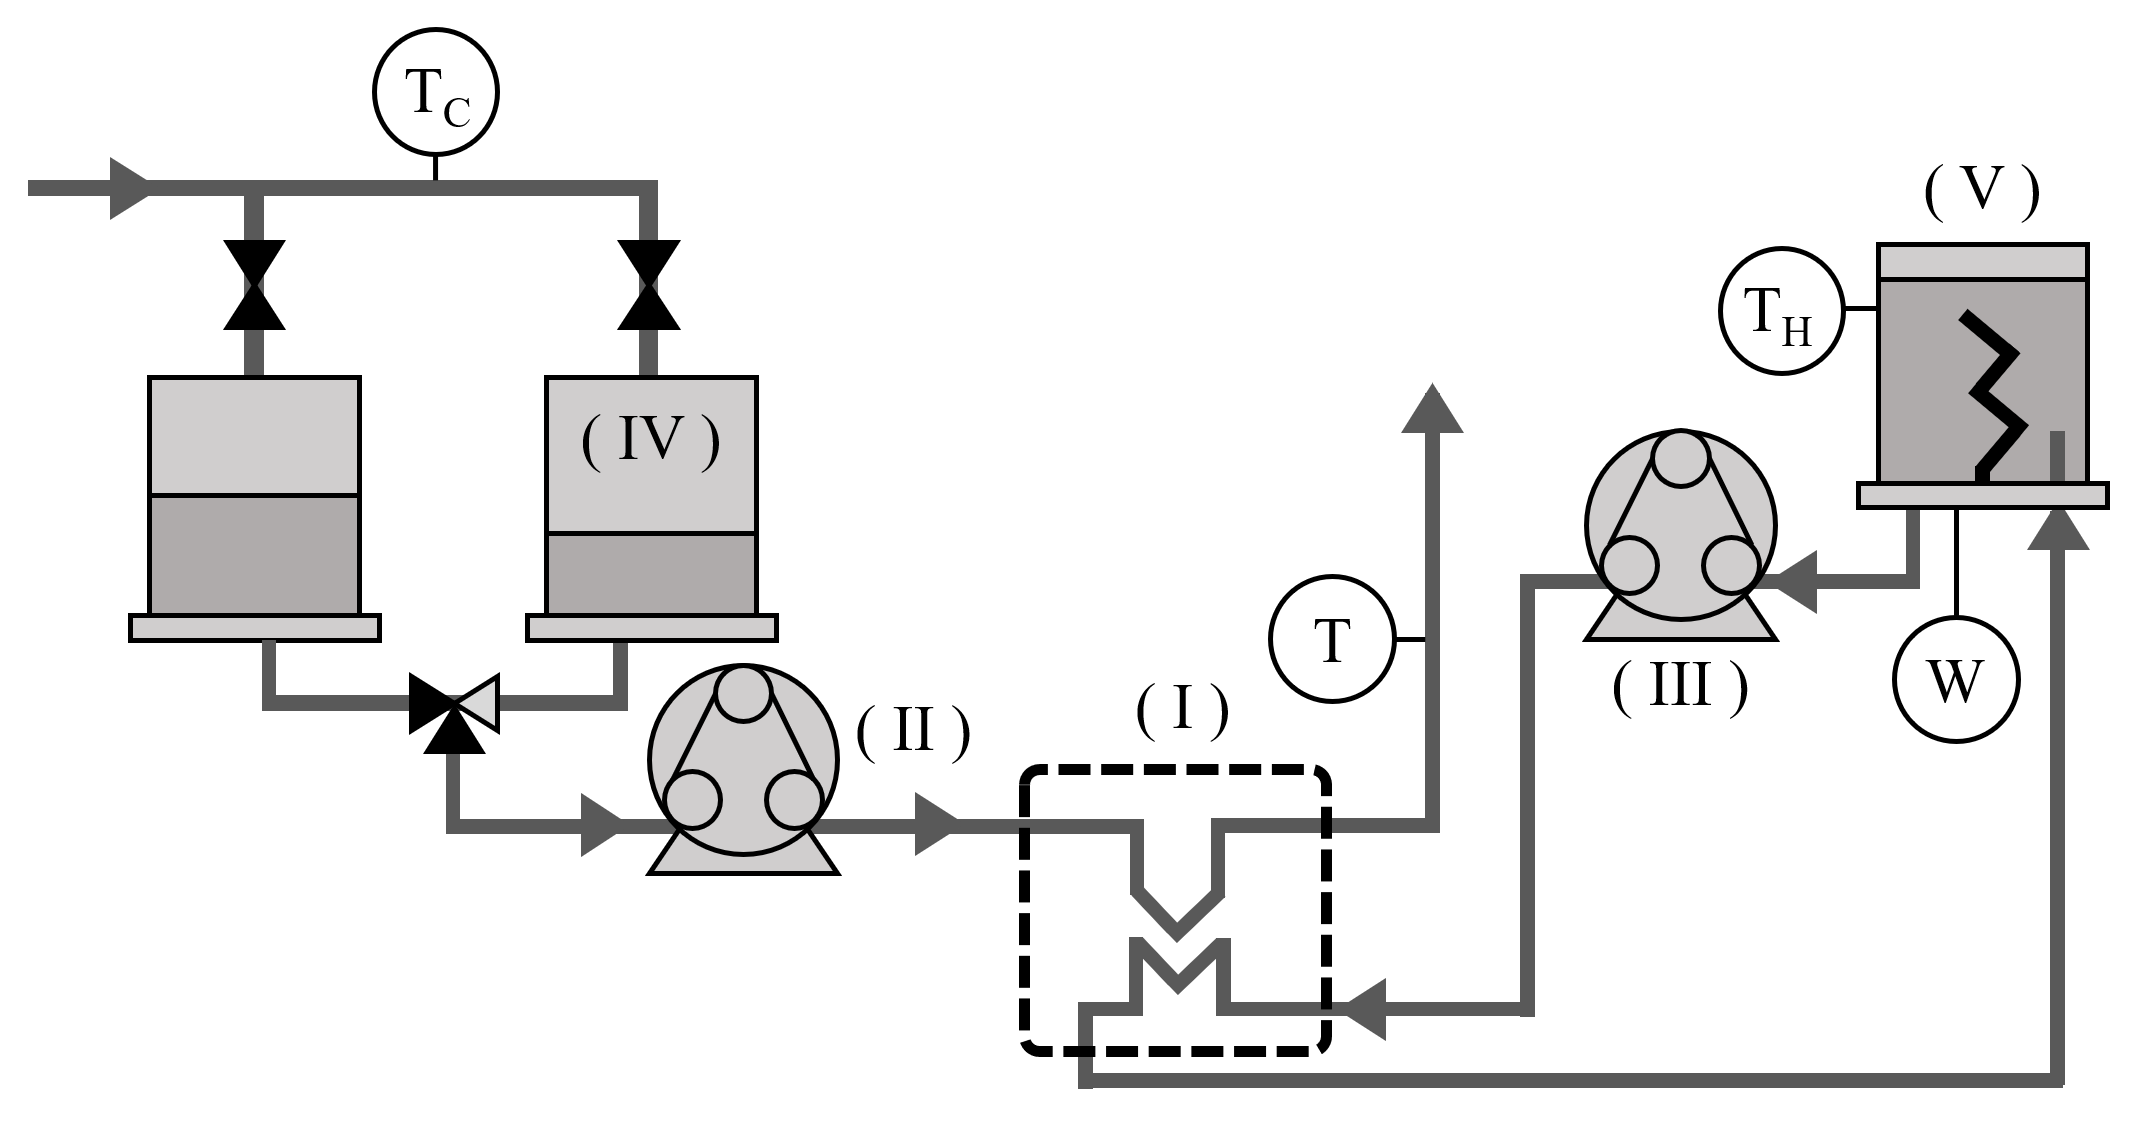
\includegraphics[width=0.8\textwidth]{images/HE_scheme}
				\caption{Scheme of Armfield PCT23. Heat exchanger (I), peristaltic pump for cold medium (II), peristaltic pump for heating medium (III), tank for cold medium (IV), heater for heating medium (V), temperature sensors ($\mathrm{T}$ -- controlled temperature, $\mathrm{T}_\mathrm{C}$ -- cold outlet cold medium temperature, $\mathrm{T}_\mathrm{H}$ -- heating medium temperature), and electric power for maintaining the temperature of the heating medium (W). }
				\label{fig:HE_scheme}
			\end{center}
		\end{figure}
	}

	\comment{
		How was it determined that Qy has the most significant effect in the heat exchange process? What constitutes "significant effect"?
	}

	\answer{
		We thank the Reviewer for pointing out insufficient discussion on the selection of the tuning penalty matrix $Q_\mathrm{y}$. By significant effect, we meant the direct association of the tuned penalty matrix with the tuning factor $\rho$, which is calculated based on the reference value. We revisited the corresponding paragraph to describe the tuning procedure.	

		
		\begin{quote}			
			\change{The penalty matrices of the problem in Eq.~(1) were systematically tuned, and the corresponding control setup was implemented on the laboratory heat exchanger for each setup of the considered explicit MPC controllers. 
			First, the tuning procedure aimed to determine which penalty matrix is the most suitable for real-time tuning. The most relevant was the penalty matrix $Q_\mathrm{y}$ as the tuning is directly associated with a reference value, which takes place in the calculation of the tuning factor $\rho$. Moreover, the tuning of $Q_\mathrm{y}$ preserved a satisfactory control performance.} Next, the boundary values of the tunable matrix $Q_\mathrm{y}$ were tuned until the following limit values were determined based on the measured closed-loop control data: $Q_\mathrm{y, L}$ = 100 and $Q_\mathrm{y, U}$ = 1\,000.			
		\end{quote}
	}

	\comment{
		In the heat exchange process, the dynamics of the hot stream appears to be neglected. Why is this the case? I am not sure about the explanation given on why different steady-state inputs are observed. The flow rate of the hot stream is adjusted so the cold stream outlet temperature is maintained at the reference value is done. It seems, though not shown, that the hot stream inlet temperature is maintained to be constant. Based on the results, it would seem that the steady-state hot stream temperature is free to vary. What about the cold stream inlet temperature? Please given the trajectories of all these variables, or at least, the temperatures. What is the impact of the repeatability of the experiments given that the hot stream temperature is allowed to vary? In any case, the metrics presented in Table 1 are reported for one experiment per scenario. I would encourage computing these metrics for several experiments to ensure repeatability of the experiments and make the results more convincing.
	}
	\answer{
		We thank the Reviewer for the very insightful comment on the experiment setup. 
		First, we would like to address the doubts about the constant steady-state values of cold and heating medium temperatures. Regarding the temperature of the cold medium, due to the limited hardware interface, it was not possible to measure the data continuously, store them, and plot the trajectory in a Figure. Nevertheless, the temperature of the cold medium was manually checked multiple times during the experiment and was constant. The advantage is that no other factor affects the temperature of the cold medium except the room temperature, which was constant. We added the information about the inlet temperature of the cold medium into the manuscript:
		
		\begin{quote}
			The heat exchanger is 90\,mm wide, 103\,mm long, and 160\,mm high. The heat exchange is performed between the cold medium (water) and the hot medium (water). The heat exchange is performed between the \change{cold medium} (water) and the hot medium (water). \change{The cold medium as well as the heating medium are transported to the heat exchanger by two peristaltic pumps with flexible tubing from silicon rubber. The flow rate of the cold medium is constant, while the aim of control is to track the reference value of the outlet cold medium temperature. Therefore, the controlled variable is the \change{cold medium} temperature $T$ at the outlet of the heat exchanger. The inlet cold medium temperature was constant during the whole control, i.e., $T_\mathrm{C} = 19^{\circ}$\,C.} 
		\end{quote}

		
		Regarding the temperature of the heating medium, we provide the corresponding trajectories of the temperature in Figure~\ref{fig:Th}. We kindly remind the Reviewer that the order of the Figures in the manuscript is different. Note that the legend corresponds to the specific setup of MPC, but the temperature of the heating medium was controlled with an auxiliary P controller with the same proportional gain in every control scenario. It can be seen that the temperature of the heating medium remains relatively constant during the whole control, except for the undershoots in the scenario with upper boundary MPC, i.e., blue trajectory. The undershoots can be easily associated with the trajectory of the voltage on the pump dosing the heating medium (and ultimately the heating medium flow rate). As the upper boundary MPC calculated ``aggressive'' control inputs, the increased flow rate of the heating medium led to a slight decline in the heating medium temperature. After approximately 100 seconds, the heating medium warmed up to the reference value, i.e., $T_{\mathrm{H, ref}} = 70^{\circ}$\,C and remained constant within the accuracy of the temperature sensor. It can be seen that although the temperature of the heating medium is constant and identical for all control scenarios (MPC setups), the value of the voltage on the pump dosing the heating medium is not the same when tracking the temperature $T_{\mathrm{ref}} = 50^{\circ}$\,C. Therefore, the same conditions were fulfilled for all control scenarios. We explain the different values of the manipulated variable with the heat accumulated inside the heat exchanger plates, and therefore, less heating medium was necessary to heat the cold medium. This phenomenon does not happen when tracking the reference value $T_{\mathrm{ref}}$ = 45\,$^{\circ}\mathrm{C}$, which originates in the nonlinear nature of the heat transfer process. When working in a higher temperature range, the gain of the heat transfer process decreases, and the sensitivity to changes in the heating medium flow is lower. Therefore, even different flow rates of the heating medium lead to the same temperature at the outlet.
		
		Next, we would like to make clear that the repeatability of the realized laboratory experiments was ensured by fixing all the relevant conditions, such as the cold medium dosed into the heat exchanger from the large retention tanks at the laboratory temperature and the constant inlet temperature of the heating medium. 
		
		Based on our answer to the Reviewer's comment, we added Figure~\ref{fig:Th} and Figure~\ref{fig:W} to the manuscript with the following explanation to give the reader an insight into the dynamics of the heating medium:
		
		\begin{quote}
			An interesting phenomenon can be observed while tracking the third reference value, i.e., $T_{\mathrm{ref}}$ = 50\,$^{\circ}\mathrm{C}$. Although the steady-state values of temperature have the same value, the values of the manipulated variable are different. To check the correctness of the results, the measurements were performed multiple times and led to the same behavior. \change{Also, the inlet temperatures of the cold and heating medium were checked to exclude the effect of a disturbance. Regarding the temperature of the cold medium, due to the limited hardware interface, it was not possible to measure the data continuously, store them, and plot the trajectory in a Figure. Nevertheless, the temperature of the cold medium was manually checked multiple times during the experiment and was constant.} 
			
			\change{Regarding the temperature of the heating medium, the corresponding trajectories of the temperature can be seen in Figure~\ref{fig:Th}, and the electric power, i.e., the corresponding manipulated variable, can be seen in Figure~\ref{fig:W}. Note that the legends correspond to the specific setup of MPC, but the temperature of the heating medium was controlled with a simple P controller with the same proportional gain in every control scenario.} 
			
			\change{It can be seen that the temperature of the heating medium remains relatively constant during the whole control, except for the undershoots in the scenario with upper boundary MPC, i.e., blue trajectory. The undershoots can be easily associated with the trajectory of the voltage on the pump dosing the heating medium (and ultimately the heating medium flow rate). As the upper boundary MPC calculated ``aggressive'' control inputs, the increased flow rate of the heating medium led to a slight decline in the heating medium temperature. After approximately 100 seconds, the heating medium warmed up to the reference value, i.e., $T_{\mathrm{H, ref}} = 70^{\circ}$\,C and remained constant within the accuracy of the temperature sensor. It can be seen that although the temperature of the heating medium is constant and identical for all control scenarios (MPC setups), the value of the voltage on the pump dosing the heating medium is not the same when tracking the temperature $T_{\mathrm{ref}} = 50^{\circ}$\,C. Therefore, the same conditions were fulfilled for all control scenarios.} 
			
			\change{The reason for this behavior} could be explained by the peak of the manipulated variable associated with the upper boundary controller at time 800\,s, see Figure~10, blue. After approximately 100\,s, the value of the manipulated variable dropped and settled at a value lower than the value associated with the lower boundary controller, see Figure~10, red. This is a consequence of the heat accumulated inside the heat exchanger plates, and therefore, less heating medium was necessary to heat the cold medium. This phenomenon does not happen when tracking the reference value $T_{\mathrm{ref}}$ = 45\,$^{\circ}\mathrm{C}$, which originates in the nonlinear nature of the heat transfer process. When working in a higher temperature range, the gain of the heat transfer process decreases, and the sensitivity to changes in the heating medium flow is lower. Therefore, even different flow rates of the heating medium lead to the same temperature at the outlet.
		\end{quote}
		

		
		  
		%We find this comment comprises three closely related points to be answered individually.
		
		%First, we confirm that the hot stream temperature is considered constant. This assumption is supported by the implementation of the auxiliary P controller dedicated to controlling the temperature in the heating tank for the hot medium. Although the control profiles of the hot stream temperature ($T = 70^{\circ}$\,C) are not provided, the corresponding dynamics was negligible and the steady-state values of the heating medium temperature were constant.
		
		%Next, we would like to make clear that the repeatability of the realized laboratory experiments was ensured by fixing all the relevant conditions, such as the cold medium dosed into the heat exchanger from the large retention tanks at the laboratory temperature and the constant inlet temperature of the heating medium.
		
		%Finally, we would like to address the doubts related to observing the varying steady-state values of the control inputs corresponding to the same value of the controlled variable - the outlet temperature of the heated medium. Although this performance may look like an error introduced during a single measurement, we realized a series of laboratory experiments to investigate this phenomenon with analogous results.
		
		%The steady-state value of control input settled either in the close neighborhood of $U = 45\,\%$, or close to the value of $U = 55\,\%$. This phenomenon was even observed with different setup of weighting matrix $R = 100$ during the initial tuning and searching for the ``right'' setup of all penalty matrices. The input variable also settled close to $U = 52\,\%$ (e.g., for $Q_{\mathrm{y}} = 1000$), or close to the value of $U = 42-45\,\%$ (e.g., for $Q_{\mathrm{y}} = 100$). Therefore, after the detailed analysis, we state that this phenomenon originates from the physical construction of the heat exchanger due to the portion of heat released from the plates for the (relatively high) reference value around $T = 50^{\circ}$\,C.
		
		\begin{figure}
			\begin{center}
				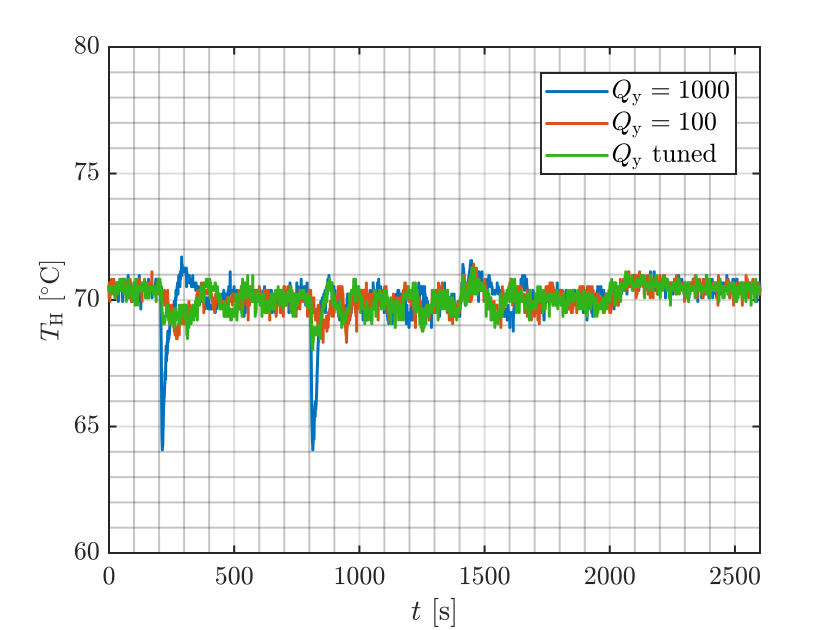
\includegraphics[width=0.7\textwidth]{images/Th}
				\caption{Auxiliary P controller: The trajectory of heating medium temperature control.}
				\label{fig:Th}
			\end{center}
		\end{figure}
	
		\begin{figure}
			\begin{center}
				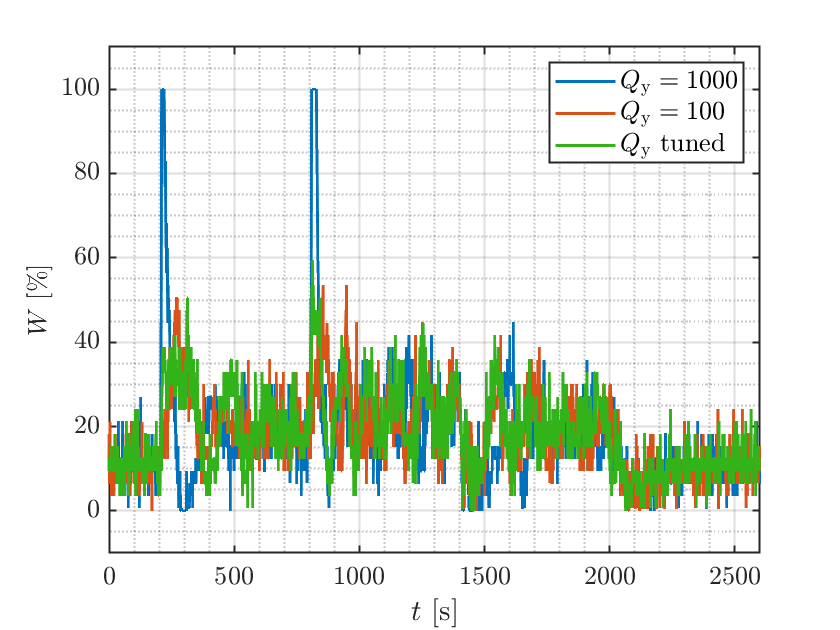
\includegraphics[width=0.7\textwidth]{images/W}
				\caption{Auxiliary P controller: The trajectory of electric power controlling the heating medium temperature.}
				\label{fig:W}
			\end{center}
		\end{figure}	

	}
	
	
	\bibliographystyle{plain}
	\bibliography{references}
	
\end{document}


